% ---------------PLANTILLA INFORMES-------------- %

%---------Preambulo-------
\documentclass[11pt,letterpaper]{extarticle}        % Clase


\usepackage[utf8]{inputenc}                      % Codificación UTF-8
\usepackage[spanish]{babel}                      % Idioma del documento
\usepackage[left=2cm,right=2cm,bottom=3cm,top=2.5cm]{geometry}  % Dimesiones


% --------------------------LIBRERIAS-------------------------- %

\usepackage{enumitem}               % Enumeracion
\usepackage{fancyhdr}               % Encabezados y pies de pagina
\usepackage[ampersand]{easylist}    % Listas
\usepackage{amsmath}                % Fórmulas matemáticas
\usepackage{amssymb}                % Símbolos matemáticos
\usepackage{caption}                % Leyendas
\usepackage{color}                  % Colores
\usepackage{fancyhdr}               % Encabezados y pié de páginas
\usepackage{float}                  % Administrador de posiciones de objetos
\usepackage{geometry}               % Dimensiones y geometría del documento
\usepackage{graphicx}               % Propiedades extra para los gráficos
\usepackage[hidelinks]{hyperref}    % Permite añadir enlaces y referencias
\usepackage[makeroom]{cancel}       % Cancelar términos en fórmulas
\usepackage[version=4]{mhchem}      % Fórmulas químicas
\usepackage{multicol}               % Múltiples columnas
\usepackage{lipsum}                 % Permite crear textos dummy
\usepackage{longtable}              % Permite utilizar tablas en varias hojas
\usepackage{listings}               % Permite añadir código fuente
\usepackage{setspace}               % Cambia el espacio entre líneas
%\usepackage{subfig}
\usepackage{subfig}              % Permite agrupar imágenes
\usepackage{titlesec}               % Cambia el estilo de los títulos
\usepackage{url}                    % Permite añadir enlaces
\usepackage{wrapfig}                % Permite comprimir imágenes
\usepackage{pdfpages}

% LIBRERÍAS DEPENDIENTES
\usepackage{epstopdf}               % Convierte archivos .eps a pdf
\usepackage{multirow}               % Añade nuevas opciones a las tablas
\makeatletter

% INFORMACIÓN DEL DOCUMENTO
\newcommand{\nombredelinforme}{Pruebas en una Máquina de
Refrigeración Mecánica}
\newcommand{\fecharealizacion}{\today}
\newcommand{\fechaentrega}{\today}
\newcommand{\nombreuniversidad}{Universidad de Chile}
\newcommand{\nombrefacultad}{Facultad de Ciencias Físicas y Matemáticas}
\newcommand{\departamentouniversidad}{Departamento de Ingeniería Mecánica}
\newcommand{\imagendeldepartamento}{images/departamentos/dimec}
\newcommand{\imagendeldepartamentoescala}{0.29}
\newcommand{\localizacionuniversidad}{Santiago, Chile}
\newcommand{\nombredelcurso}{Laboratorio de Máquinas}
\newcommand{\codigodelcurso}{ME5301}



% CONFIGURACIONES
\newcommand{\tiporeferencias}{apa}                  % Tipo de referencias
\newcommand{\nombreltformulas}{Lista de Fórmulas}   % Nombre de la lista de fórmulas
\newcommand{\nombrelttablas}{Lista de Tablas}       % Nombre de la lista de tablas
\newcommand{\nombreltfiguras}{Lista de Figuras}     % Nombre de la lista de figuras
\newcommand{\nombreltcontend}{Índice de Contenidos} % Nombre del índice de contenidos
\newcommand{\nombreltwtablas}{Tabla}                % Nombre de las tablas
\newcommand{\nombreltwfigura}{Figura}               % Nombre de las figuras
\numberwithin{equation}{section}                    % Ecuaciones con numero de seccion

% -------------------------FUNCIONES ESPECIALES------------------------- %
\newcommand{\grados}{^{\circ}}                      % Circulo superior para grados
\newcommand{\quotes}[1]{``#1''}                     % Citas
\newcommand{\quotesit}[1]{\textit{\quotes{#1}}}     % Citas italico

% ------ FORMATO ------------%

\fancypagestyle{Portada}{
\fancyhead[L] {\nombreuniversidad \\ \nombrefacultad \\ \nombredelcurso \: \codigodelcurso }
\fancyhead[R]{\includegraphics[scale=\imagendeldepartamentoescala]{\imagendeldepartamento}}
\cfoot{}
}

\fancypagestyle{NoPortadaNoEnumerada}{
\fancyhead[L] {\nombredelcurso \: \codigodelcurso \\ \nombredelinforme}
\fancyhead[R]{\nombreuniversidad \\ \departamentouniversidad}
\cfoot{}
}

\fancypagestyle{NoPortada}{
\fancyhead[L] {\nombredelcurso \: \codigodelcurso \\ \nombredelinforme}
\fancyhead[R]{\nombreuniversidad \\ \departamentouniversidad}
\cfoot{\thepage}
}






% --------------------------------DOCUMENTO-------------------------------- %
% INICIO DEL DOCUMENTO
\begin{document}

%BEGIN_FOLD
% PORTADA
\newpage
\pagestyle{fancy}
\thispagestyle{Portada}
\vspace*{5cm}
\begin{center}
	\vspace{1cm}
	\noindent\rule{\linewidth}{0.4pt}\\
	\Huge {\textbf{\nombredelinforme}}
		\vspace{0.3cm} 
	\noindent\rule{\linewidth}{0.3pt}
\end{center}
\vfill

% INTEGRANTES, PROFESORES Y FECHAS
\begin{minipage}{0.965\textwidth}
	\begin{flushright}
		\begin{tabular}{ll}
			Alumno: 
				& \begin{tabular}[t]{@{}l@{}}
					Daniel Mardini González\\
				\end{tabular} \\
			Curso:
				& \nombredelcurso \\
			Código:
				& \codigodelcurso \\
			Profesor: 
				& \begin{tabular}[t]{@{}l@{}}
					Ricardo Díaz S.\\
				\end{tabular} \\
			
			\multicolumn{2}{l}{Ayudante del laboratorio: Pedro Pino T.} \\
			& \\
			\multicolumn{2}{l}{Fecha de entrega: \fechaentrega} \\
			\multicolumn{2}{l}{\localizacionuniversidad}
		\end{tabular}
	\end{flushright}
\end{minipage}

% CONFIGURACIÓN DE PÁGINA Y ENCABEZADOS
\newpage
\renewcommand{\listfigurename}{\nombreltfiguras}    % Nombre del índice de figuras
\renewcommand{\listtablename}{\nombrelttablas}      % Nombre del índice de tablas
\renewcommand{\contentsname}{\nombreltcontend}      % Nombre del índice
\renewcommand{\tablename}{\nombreltwtablas}         % Nombre de la leyenda de las tablas
\renewcommand{\figurename}{\nombreltwfigura}        % Nombre de la leyenda de las figuras

\numberwithin{equation}{section}
\numberwithin{table}{section}
\numberwithin{figure}{section}


\pagestyle{fancy}
\thispagestyle{NoPortadaNoEnumerada}

% TABLA DE CONTENIDOS
\newpage
\tableofcontents        % Tabla de contenidos
\newpage
\listoffigures          % Índice de figuras
\listoftables           % Índice de tablas


\newpage
\setcounter{page}{1}
\pagestyle{NoPortada}

\section{Introducción}
Es parte del día a día abrir el refrigerador y sentir que los alimentos en su interior se mantienen a una baja temperatura pero ¿cómo se les extrae el calor?. La respuesta es un sistema de refrigeración mecánica. Estos aparatos funcionan recibiendo trabajo mediante un compresor para modificar las propiedades de un fluido de trabajo llamado refrigerante que entra en contacto térmico con los elementos a enfriar y extrae su energía.\\

En el presente documento se encuentra un estudio termodinámico del sistema de Refrigeración mecánica del laboratorio de máquinas del departamento de Ingeniería Mecánica de la Universidad de Chile. Para ello se toman medidas tanto de propiedades del refrigerante como de variables que pertenecen a los equipos periféricos. Con esos datos se calculan valores incógnitos que no se midieron directamente, además de diferentes coeficientes que dan cuenta del rendimientos del aparato. Finalmente se extrae el diagrama P-h (Presión-Entalpía) que caracteriza al sistema.

\section{Objetivos}
\subsection*{Objetivo principal}
\begin{itemize}
\item Estudiar el funcionamiento  y componentes de un sistema de refrigeración mecánica
\end{itemize}
\subsection*{Objetivos secundarios}
\begin{itemize}
\item Conocer el ciclo teórico y real del sistema.
\item Realizar pruebas y tomar medidas en la máquina de refrigeración.
\item Obtener el ciclo termodinámico que sigue el fluido en el equipo de refrigeración del laboratorio.
\end{itemize}

\section{Antecedentes}
A continuación se presentan los conceptos y antecedentes clave para comprender el sistema a estudiar.

\subsection{Freón 12}
El fluido de trabajo que se utiliza en el sistema corresponde al freón 12 o refrigerante R12 que es un gas incoloro a temperatura ambiente, se vaporiza fácilmente a esta temperatura. Tiene un punto de fusión muy bajo de -158 $\grados$C y un punto de ebullición de -30$\grados$C. El líquido tiene una densidad de $1.486$[g/cm$^3$]. La curva de saturación de este refrigerante se encuentra en la tabla \ref{t:Freon12Saturacion} del anexo.

\subsection{Entalpía}
La entalpía $h$ se define como la combinación o suma de la energía interna de un sistema con su flujo de trabajo\cite[p.11]{b:Produccion} bajo la siguiente ecuación:

\begin{equation}
\label{e:Entalpia}
h = u + Pv
\end{equation}

Donde $u$ es la energía interna, $P$ es la presión y $v$ es el volumen específico del sistema. Existen tablas que relacionan este valor con distintas propiedades como la Temperatura y la Presión de un fluido.

\subsection{Calor específico}
El calor específico $c$ corresponde a la cantidad de energía que se le debe suministrar a un sistema para aumentar una unidad de Temperatura por unidad de masa\cite[p.46]{b:Produccion}. La definición se traduce en la ecuación \ref{e:CalorEspecifico}, en donde $q$ es energía absorbida por unidad de masa y $T$ la temperatura del sistema.
\begin{equation}
\label{e:CalorEspecifico}
c = \frac{dq}{dT}
\end{equation}
Integrando la ecuación \ref{e:CalorEspecifico}, suponiendo $c$ constante en el cambio de temperatura y multiplicando por la masa $m$ se obtiene que:

\begin{equation}
\label{e:Energia}
Q = m c\Delta T
\end{equation}



\subsection{Calor}
El calor $\dot{Q}$ se entiende como la energía que fluye a raiz de una diferenecia de temperatura \cite[p.5]{b:Produccion}. El calor se relaciona con la entalpía y el calor específico mediante las ecuaciones 
\ref{e:CalorEntalpia} y \ref{e:CalorCalor} respectivamente. En ambos casos $\dot{m}$ corresponde al flujo másico.

\begin{equation}
\label{e:CalorEntalpia}
\dot{Q} = \dot{m} \Delta h
\end{equation}

\begin{equation}
\label{e:CalorCalor}
\dot{Q} = \dot{m} c \Delta T
\end{equation}

\subsection{Ciclo termodinámico}
El sistema pasa por una serie de estados cíclicos que corresponden a los mismos que tiene una bomba de calor pero para el caso de la refrigeración mecánica, los puntos son recorridos en sentido inverso. Se explicará en primera instancia el ciclo de Carnot que corresponde al ciclo ideal de una máquina térmica y luego se verá el ciclo real del proceso.

\begin{figure}
\centering
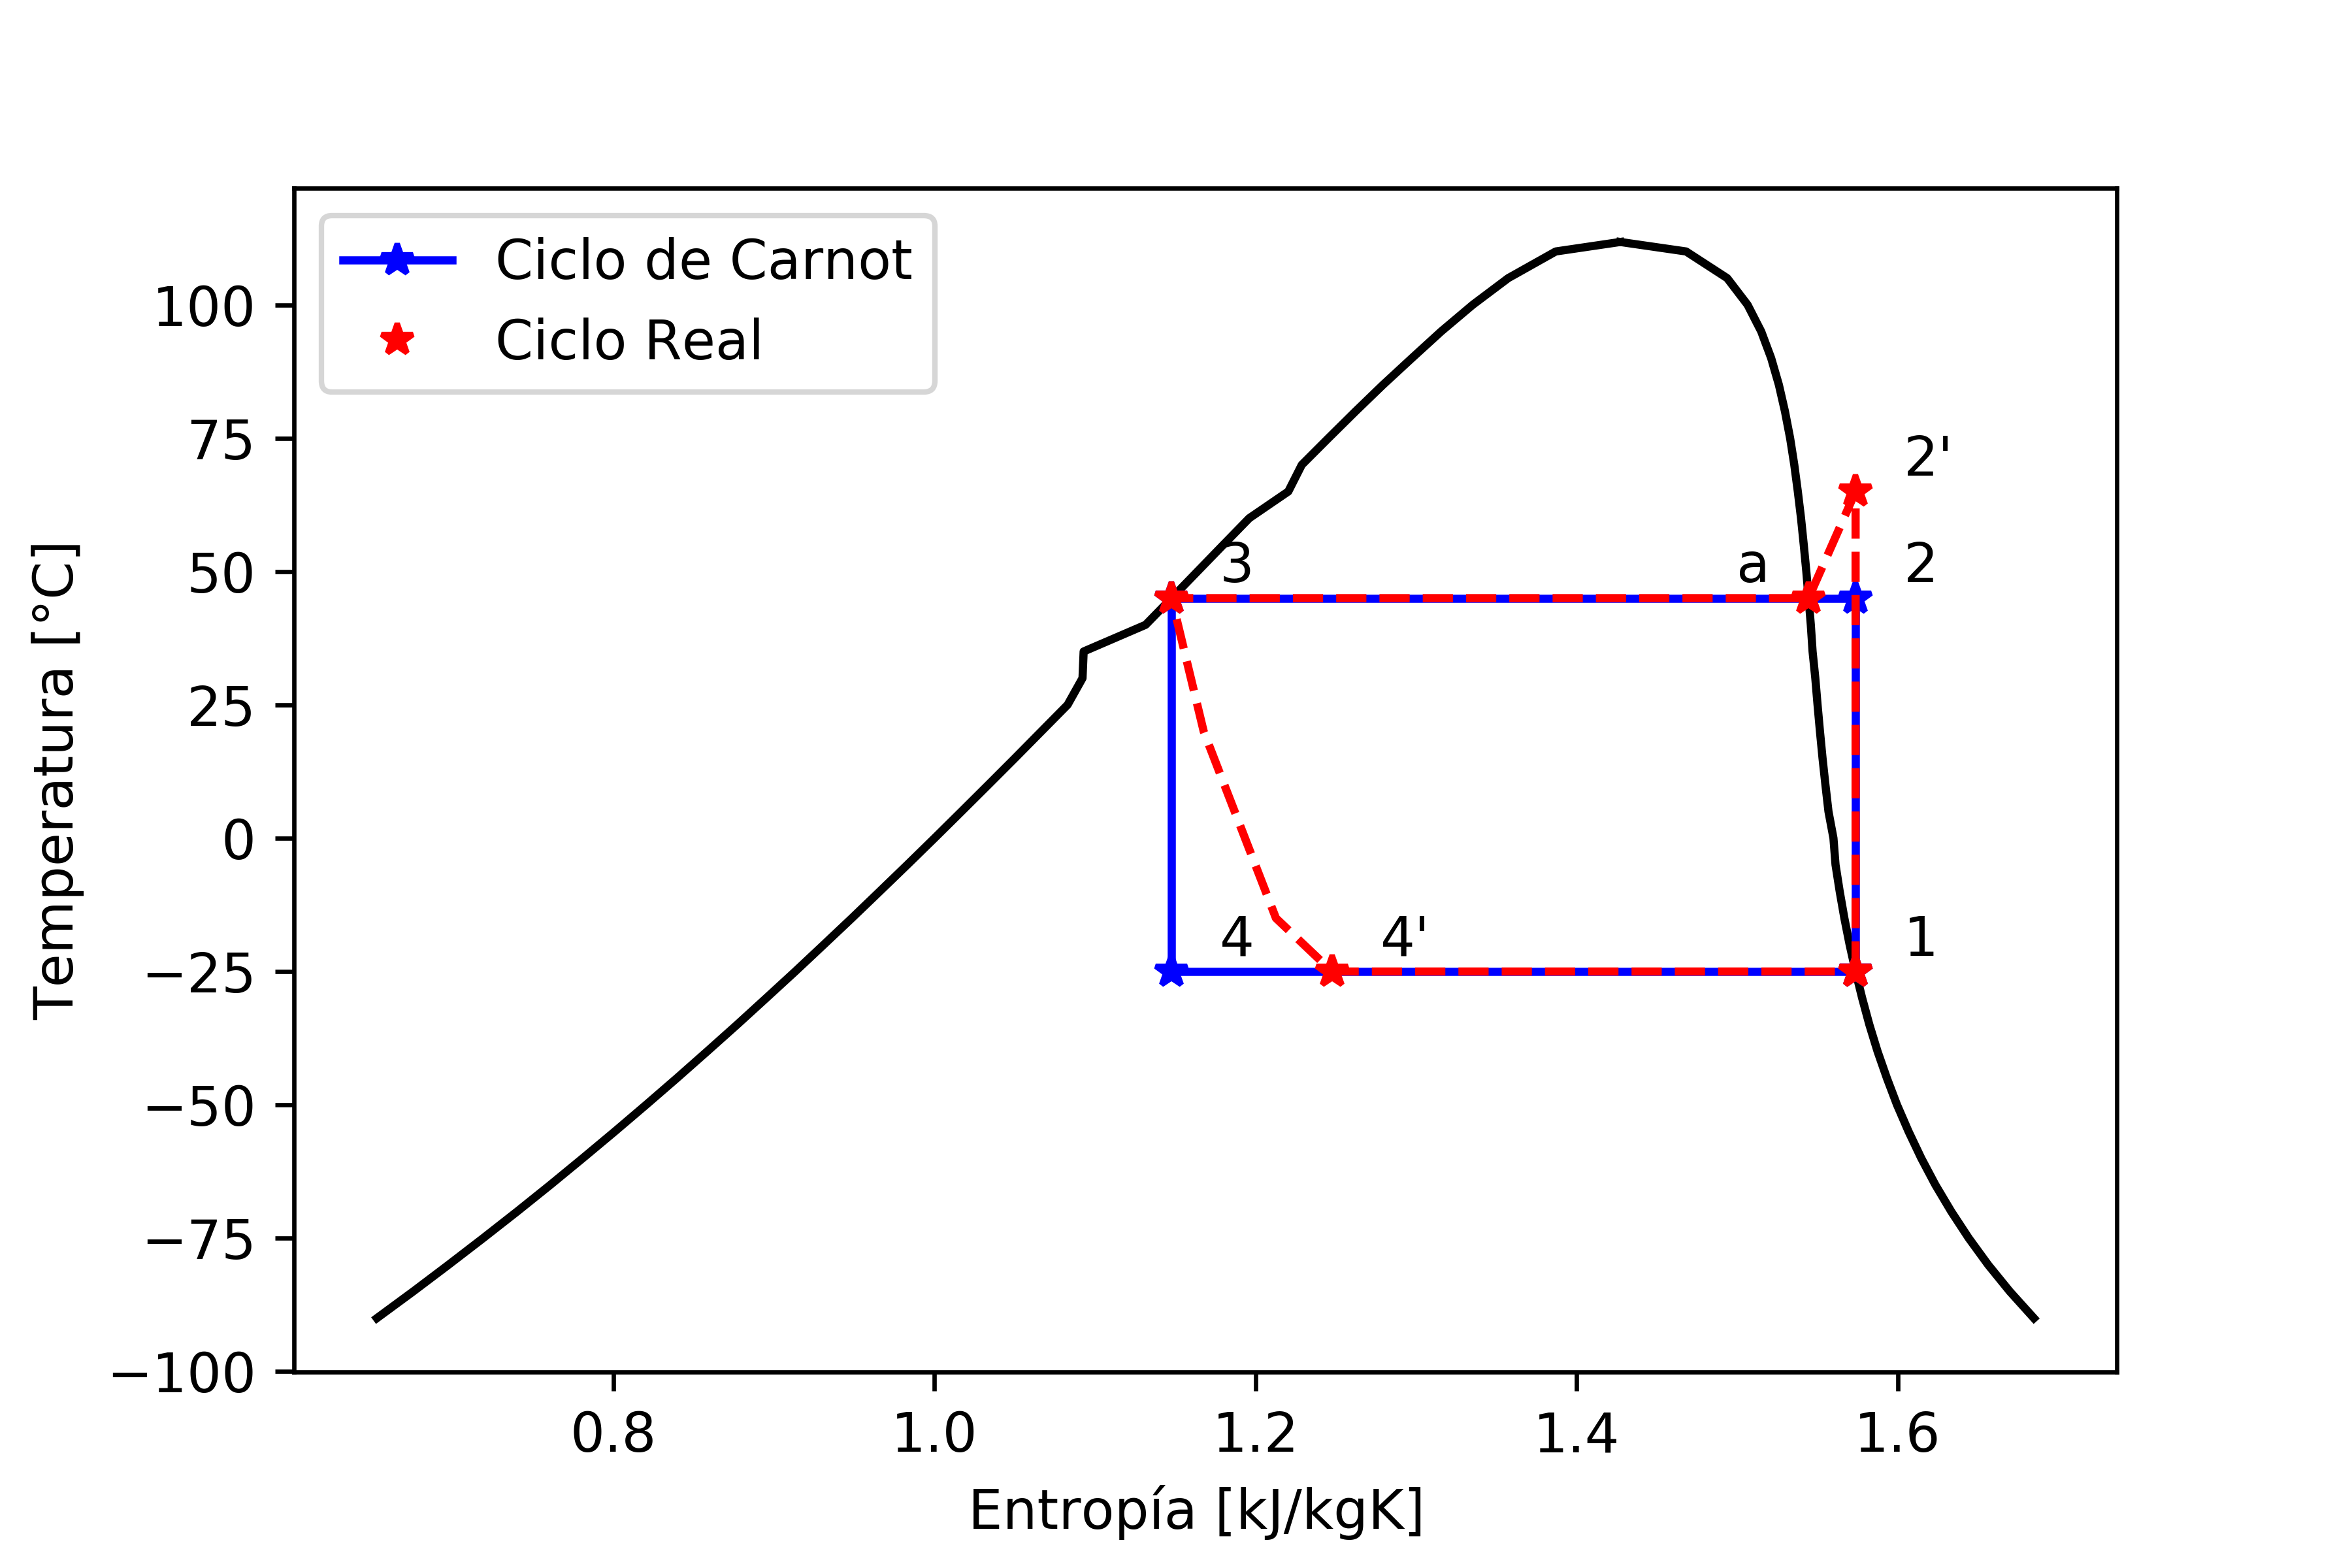
\includegraphics[width=0.7\linewidth]{Anexo/DiagramaTs}
\caption{Diagrama T-s del ciclo}
\label{f:Ts}
\end{figure}

\subsection*{Ciclo de Carnot}
En la figura \ref{f:Ts} se aprecian 2 ciclos termodinámicos, el primero, marcado por los puntos 1-2-a-3-4, corresponde al ciclo de Carnot. Este recorrido consta de distintas etapas:
\begin{itemize}
\item 1-2) Compresión isoentrópica en una compresor.
\item 2-a) Compresión isotérmica en compresor.
\item a-3) Condensación (isotérmico) en un condensador.
\item 3-4) Expansión isoentrópica.
\item 4-1) Evaporación (isotérmico) en un evaporador.
\end{itemize}
Hay que tener en cuenta que en el tramo 4-1 el fluido se evapora absorbiendo calor del medio. La eficiencia $e$ del ciclo de refrigeración de Carnot se define como por la razón entre el este calor absorbido $Q_e$ y el trabajo $W$ entregado por los compresores al fluido:
\begin{equation}
e = \frac{Q_e}{W} = \frac{T_1}{T_2-T_1}
\label{e:eficiencia}
\end{equation}

\subsubsection*{Ciclo Real}
Los puntos 1-2'-a-3-4' corresponden al ciclo real de refrigeración mecánica, este ciclo es menos eficiente que el ciclo de Carnot, es decir, requiere más trabajo para absorber el mismo calor, y las modificaciones realizadas se deben a las limitaciones técnicas de los equipos existentes: No se tienen compresores isotérmicos y la expansión se realiza en una válvula de expansión isoentálpica. El ciclo corresponde a:
\begin{itemize}
\item 1-2') Compresión isoentrópica en una compresor.
\item 2'-a) Expansión isoentálpica en válvula de expansión.
\item a-3) Condensación (isotérmico) en un condensador.
\item 3-4') Expansión isoentálpica en válvula.
\item 4'-1) Evaporación (isotérmico) en un evaporador.
\end{itemize}

\subsection{Equipo}
Para realizar la experiencia se encuentra un sistema de refrigeración mecánica en el laboratorio de máquinas del departamento de Ingeniería Mecánica de la Universidad de Chile. El equipo se puede apreciar en la figura \ref{f:Equipo} y se encuentra esquematizado en la figura \ref{f:Esquema}, y consiste principalmente en un circuito cerrado para el Freón que cambia de estado en las distintas etapas, un circuito con un caudal de agua que permite ser medido mediante un estanque graduado y un circuito electrico que disipa calor a través de una resistencia. los componentes del aparato simulan una situación de refrigeración:

\begin{itemize}
\item El condensador corresponde a un intercambiador de calor entre el refrigerante y el agua. Esta última es depositada en un estanque de $30\times30$ de base para el registro del caudal.
\item La válvula de expansión reduce la presión del Freón líquido para que ingrese al evaporador.
\item El evaporador consiste en un intercambiador de calor entre el refrigerante y la resistencia, los cuales están inmersos en una cuba y se dispone de una termocupla para medir la temperatura del sistema, además se puede medir el voltaje y la corriente que se le aplica a la resistencia mediante el uso de multímetros.
\item La compresión se realiza en un compresor de pistón que es alimentado por un motor eléctrico del que se tiene registro de su potencia mediante un Wattmetro y dos manómetros que permiten conocer las presiones de entrada y salida.
\end{itemize}

\begin{figure}[H]
\begin{minipage}[t]{.45\textwidth}
\centering
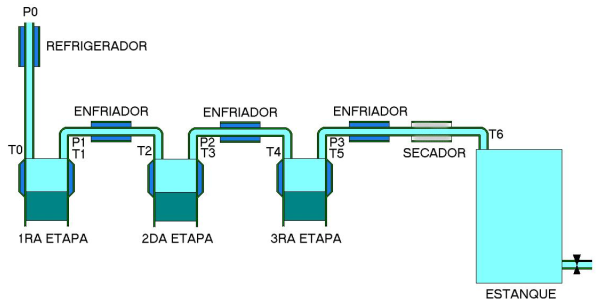
\includegraphics[width=\linewidth]{Equipo}
\caption{Equipo disponible en el laboratorio}
\label{f:Equipo}
\end{minipage}
\hfill
\begin{minipage}[t]{.5\textwidth}
\centering

\includegraphics[width=\linewidth]{Esquema}
\caption{Esquema general del sistema}
\label{f:Esquema}
\end{minipage}
\end{figure}


\section{Metodología}

El equipo cuenta, como se aprecia en la figura \ref{f:Equipo}, con una serie de sensores que permiten conocer distintas propiedades del fluido y los componentes y se encuentra encendido desde antes que se realicen las mediciones de modo que el sistema se encuentre en régimen permanente. Los datos que se registran durante la experiencia son:

\begin{itemize}
\item Las presiones de entrada y salida del compresor ($P_{e,comp}$y $P_{s,comp}$ respectivamente) 
\item Temperatura de entrada al evaporador $T_{e,evap}$
\item Temperatura de entrada y salida del agua del condensador ($T_{e,H_2O}$ y $T_{s,H_2O}$ respectivamente)
\item El voltaje ($V$) y la intensidad de corriente ($I$) de la resistencia
\item La potencia consumida por el compresor $P_{motor}$.
\item Se toma el tiempo $t$ que tarda el agua en llenar 10[cm] del balde.
\end{itemize}




\section{Memoria de cálculo}
Para conocer completamente los puntos que describen el ciclo se requiere calcular las entalpías $h_{i,k}$ asociadas a cada etapa del sistema. El subíndice $k$ de la entalpía corresponde a la etapa, siendo $cond$ correspondiente al condensador y $evap$ correspondiente al evaporador. El subíndice $i$ indica con una $e$ si corresponde a la entrada de la etapa y $s$  si corresponde a una salida.

\subsection{Condensador}
Se hace un balance de energía en el condensador considerando que los fluidos no se mezclan y no hay fugas, por lo tanto se tiene que los flujos másicos del Freón 12 y el agua ($\dot{m}_F$ y $\dot{m}_{H_2O}$ respectivamente) se mantienen constantes a lo largo de esta etapa y, en todo el circuito. El balance resulta que el calor $\dot{Q_1}$ cedido por el agua (y absorbido por el Freón) es:

\begin{equation}
\label{e:Q1}
\dot{Q_1} = \dot{m}_{H_2O} \cdot c_{H_2O} \cdot (T_{s,H_2O}-T_{e,H_2O}) = \dot{m}_F (h_{e,cond} - h_{s,cond})
\end{equation}

\subsection{Válvula de expansión}
La válvula de expansión reduce la presión de manera isoentálpica, de manera que la entalpía en la salida del condensador y en la entrada del evaporador son la misma.

\begin{equation}
\label{e:Valvula}
h_{s,cond} = h_{e,evap}
\end{equation}

\subsection{Evaporador}
Se hace un balance de energía en el evaporador en donde se encuentra la resistencia disipando calor $\dot{Q}_2$, cuantificado como:

\begin{equation}
\label{e:Q2}
\dot{Q}_2 = \eta \cdot V \cdot I
\end{equation}

Con $\eta$ un factor de corrección o \quotes{rendimiento} considerado $\eta = 0.86$.
Este calor $\dot{Q_2}$ es absorbido y cedido por el refrigerante, esto está determinado por el ecuación \ref{e:CalorCalor} como:

\begin{equation}
\label{e:Q22}
\dot{Q_2} = \dot{m}_F (h_{s,evap} - h_{e,evap})
\end{equation}

\subsection{Compresor}
Se realiza un balance de energía en el compresor y se obtiene que el trabajo ($\dot{W}$) que entrega el compresor al fluido es igual al cambio de sus entalpías.

\begin{equation}
\label{e:Compresor}
\dot{W} = \dot{m}_F \cdot (h_{s,comp}-h_{e,comp}) 
\end{equation}

\subsection{Cálculo general}
Al dividir las ecuaciones \ref{e:Q1} y \ref{e:Q22} se obtiene la relación:
\begin{equation}
\label{e:Relacion}
\frac{\dot{Q_1}}{\dot{Q_2}} =
\frac{\dot{m}_{H_2O} \cdot c_{H_2O} \cdot (T_{s,H_2O}-T_{e,H_2O})}{\eta \cdot V \cdot I} = 
\frac{\cancel{\dot{m}_F} (h_{e,cond} - h_{s,cond})}{\cancel{\dot{m}_F} (h_{s,evap} - h_{e,evap})} 
\end{equation}

De la ecuación \ref{e:Relacion} se tienen los valores necesarios para calcular todas las entalpías excepto $h_{s,cond}$ y $h_{e,evap}$ . Utilizando la ecuación \ref{e:Valvula} y definiendo $\alpha = \frac{\dot{Q_1}}{\dot{Q_2}}$ se despeja:
\begin{equation}
\label{e:Hbuscada}
h_{s,cond} = h_{e,evap} =
\frac{h_{e,cond}-\alpha \cdot h_{s,evap}}{1-\alpha}
\end{equation}

Se utiliza la tabla \ref{t:Resultados} para ingresar a las tablas \ref{t:Freon12-340} - \ref{t:Freon12-700-2}. Se realiza una conversión de unidades y se obtienen los resultados de la tabla \ref{t:Compresor}. Se calcula el caudal de agua con los datos de la tabla \ref{t:Resultados} y la densidad de la tabla \ref{t:Agua} con una temperatura media $T=27[\grados C]$ como:

$$ \dot{m}_{H_2O} = \frac{\text{Volumen de estanque}}{\text{Tiempo de llenado}}\times\text{Densidad}=\frac{ 30 \times 30 \times 10 \times 10^{-6} [\text{m}^3]}{278[s]} 996.6\left[\frac{kg}{m^3}\right]$$

$$ \dot{m}_{H_2O}
=0.032264\left[\frac{kg}{s}\right]$$

De la tabla \ref{t:Agua} se interpola el valor para una temperatura media $T=27[\grados C]$, obteniendo un valor del calor específico del agua $c_p = 4180.4[J/kgK]$. Reemplazando esto y los valores conocidos de la tabla \ref{t:Resultados} enla ecucaion \ref{e:Relacion} se obtiene que:

$$ \alpha =\frac{\dot{Q_1}}{\dot{Q_2}}=
\frac{\dot{m}_{H_2O} \cdot c_{H_2O} \cdot (T_{s,H_2O}-T_{e,H_2O})}
{\eta \cdot V \cdot I}=
\frac{0.032264 \times 4180.4 \times (30-24)[W]}
{0.86\times 167 \times 3.3 [W]}
=\frac{809.259}{473.946}
 $$
 
$$\alpha = 1.70749$$

Finalmente con este valor de $\alpha$ y la ecuación \ref{e:Hbuscada} se determina el valor de $h_{e,evap}$ de la siguiente manera:

$$h_{e,evap} =
\frac{h_{e,cond}-\alpha \cdot h_{s,evap}}{1-\alpha}=
\frac{369.227-1.70749 \times 365.191}{1-1.70749}\left[\frac{kJ}{kg}\right]
$$

$$h_{e,evap} = 359.486\left[\frac{kJ}{kg}\right]$$

Una vez conocidas las entalpías en el evaporador se procede a trabajar con la ecuación \ref{e:Q22} para conocer el flujo másico del Freón 12 en el circuito:

$$
\dot{m}_F = \frac{\dot{Q_2}}{(h_{s,evap} - h_{e,evap})} = 
\frac{473.946[W]}{1000\times(365.191 - 359.486)[J/kg]} 
$$

$$
\dot{m}_F = 0.083076 \left[ \frac{kg}{s}\right]
$$

\subsection{Rendimientos}
Se define el rendimiento de la refrigeración $e$ como la relación entre la potencia entregada por la resistencia y el calor absorbido por el refrigerante, básicamente.

\begin{equation}
\label{e:e}
e = \frac{\eta \cdot V \cdot I}{\dot{m}_F(h_{e,cond}-h_{s,evap})}
\end{equation}

Utilizando la ecuación \ref{e:e} y los resultados obtenidos se llega a:
$$
e = \frac{\eta \cdot V \cdot I}{\dot{m}_F(h_{e,cond}-h_{s,evap})} =
\frac{0.86 \times 167 \times 3.3[W]}{0.083076 \times(369.227-365.191)\times 1000[W]}
$$
$$e = 1.41352$$

La eficiencia real $e_{real}$ se define como la razón entre el calor absorbido por el refrigerante y la potencia que posee el motor

\begin{equation}
\label{e:ereal}
e_{real} = \frac{\eta \cdot V \cdot I}{P_{motor}\cdot \eta}
\end{equation}

De igual manera, al reemplazar los valores conocidos en la ecuación \ref{e:ereal} se obtiene:
$$e_{real} = \frac{\eta \cdot V \cdot I}{P_{motor}\cdot \eta} =
\frac{0.86 \times 167 \times 3.3[W]}
{470 \times 0.86[W]}$$

$$e_{real}= 1.17255$$

El rendimiento conjunto motor-compresor $e_{m-c}$se define como la razón entre el calor neto absorbido por el refrigerante y la potencia del motor.

 \begin{equation}
\label{e:emc}
e_{m-c} = \frac{\dot{m}_F(h_{e,cond}-h_{s,evap})}{P_{motor}\cdot \eta}
\end{equation}

Se encuentra, entonces el rendimiento conjunto reemplazando en la ecuación \ref{e:emc}:

$$
e_{m-c} = \frac{\dot{m}_F(h_{e,cond}-h_{s,evap})}{P_{motor}\cdot \eta}=
\frac{0.083076 \times(369.227-365.191)\times 1000[W]}{470\times 0.86[W]}
$$
$$
e_{m-c} = 0.829527
$$
\section{Resultados}
\begin{table}[H]
\centering
\caption{Mediciones tomadas}
\label{t:Resultados}
\resizebox{\textwidth}{!}{
\begin{tabular}{|c|c|c|c|c||c|c|c||c|c|c|}
\hline	
\multicolumn{5}{|c||}{Compresor}                                   & \multicolumn{3}{c||}{Cuba} & \multicolumn{3}{c|}{Condensador} \\
\hline \hline
$P_{motor}${[}W{]} & $P_{e,comp}[kg/cm^2]$ & $P_{s,comp}[kg/cm^2]$ & $T_{e,comp}[\grados C]$   & $T_{s,comp}[\grados C]$   & $V[V]$       & $I[A]$       & $T_{e,evap}[\grados C] $   & $T_{e,H_2O}[\grados C]$      & $T_{s,H_2O}[\grados C]$      & $t[s]$      \\
\hline
470               & 3.5                      & 7  & 20.4 & 33.5 & 167     & 3.3     & 0    & 24      & 30      & 278        \\
\hline
\end{tabular}
}
\end{table}

\begin{table}[H]
\centering
\caption{Resumen de Presiones y entalpías}
\label{t:Compresor}
\begin{tabular}{|l|c|c|c|c|}
\hline
\multicolumn{1}{|l}{} & \multicolumn{1}{l}{Compresor} & \multicolumn{1}{l}{Condensador} & \multicolumn{1}{l}{Válvula} & \multicolumn{1}{l|}{Evaporador} \\
\hline
\multicolumn{1}{|l}{Etapa} & \multicolumn{1}{l}{1} & \multicolumn{1}{l}{2} & \multicolumn{1}{l}{3} & \multicolumn{1}{l|}{4} \\
P {[}kg\textbackslash{}cm$^2${]} & 3.5 & 7.0 & 7.0 & 3.5 \\
P {[}kPa{]} & 343.233 & 686.466 & 686.466 & 343.233 \\
$h${[}kJ/kg{]} & 365.191 & 369.227 & 359.486 & 359.486\\
\hline
\end{tabular}
\end{table}


\begin{table}[H]
\centering
\caption{Resumen de flujos másicos}
\label{t:masa}
\begin{tabular}{|c|c|c|}
\hline
Fluido              & Agua     & Freón    \\ \hline\hline
$\dot{m}${[}kg/s{]} & 0.032264 & 0.083076 \\ \hline
\end{tabular}
\end{table}

\begin{table}[H]
\centering
\caption{Resumen de rendimientos}
\label{t:Rendimientos}
\begin{tabular}{|c|c|}
\hline
Rendimiento & Valor    \\ \hline\hline
$e$         & 1.41352  \\ 
$e_{real}$  & 1.17255  \\ 
$e_{m-c}$   & 0.829527 \\ \hline
\end{tabular}
\end{table}

Con la tabla \ref{t:Compresor} se arma el diagrama P-h de la figura \ref{f:Ph}.

\begin{figure}[H]
\centering
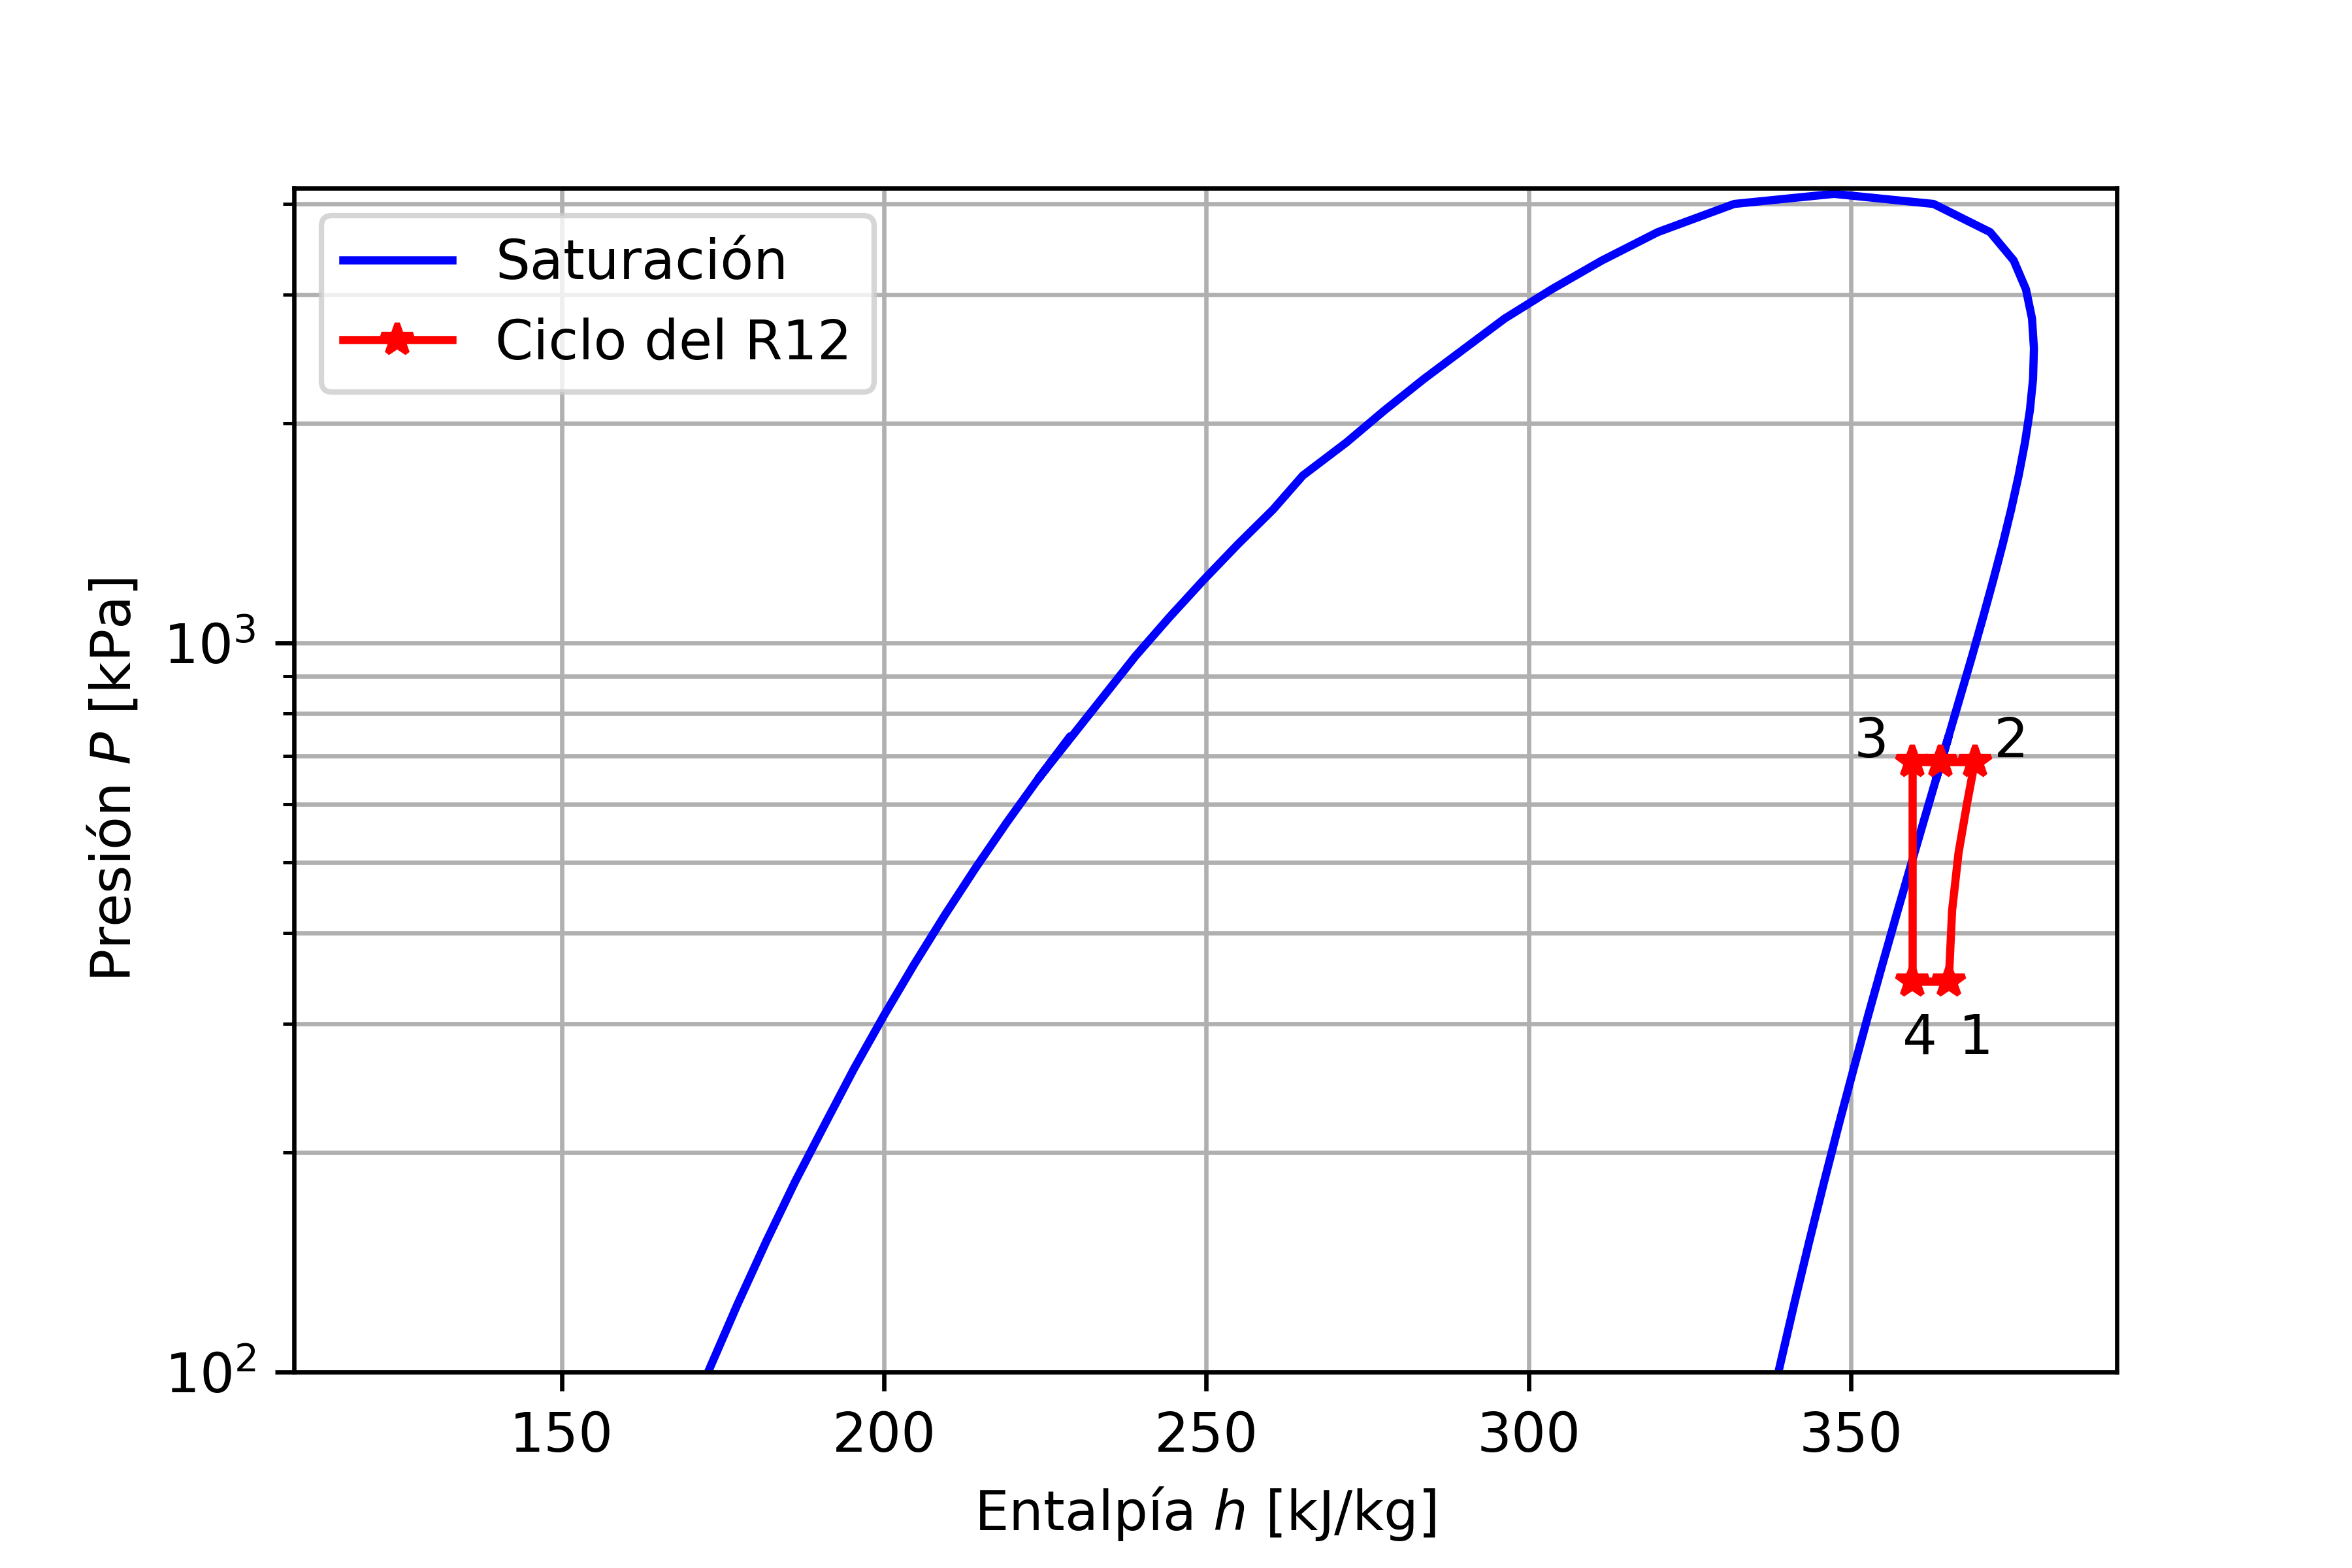
\includegraphics[width=0.6\linewidth]{Anexo/Ph}
\caption{Diagrama P-h del ciclo}
\label{f:Ph}
\end{figure}

\section{Análisis de resultados}

De los resultados el más sencillo de analizar y que resume gran parte de los demás corresponde al diagrama P-h de la figura \ref{f:Ph} pues es ahí donde se puede seguir con facilidad la ubicación del refrigerante con respecto a la linea de saturación. En este diagrama se puede observar una discordancia con lo esperado pues, idealmente, el condensador debe retornar un fluido saturado a la salida de modo que se absorba más energía y este enfríe de mejor manera el sistema objetivo.\\

Las causas de este diagrama pueden ser variadas. En una primera instancia se puede pensar en la temperatura del agua, como se ve en la tabla \ref{t:Resultados}, el líquido ingresa al intercambiador a una temperatura cercana a la temperatura ambiente (24$\grados C$) siendo que el refrigerante, según esa misma tabla, ingresa a 33.5$\grados C$. Por lo tanto una solución a esto, para mejorar el sistema, consistiría en ingresar agua a menor temperatura al condensador de modo que el refrigerante pueda realmente condensarse.\\

Una segunda fuente de error es la medición misma. La toma de datos puede afectarse si hay sensores defectuosos o mal conectados y como hay valores que se han calculado en base a estas malas mediciones, dichos datos no serían correctos. En este caso no se tiene como comprobar las mediciones pues se desconoce cuándo y cómo fue la última calibración y tampoco se tiene otra medida alternativa que sirva para comparar. Otra fuente de error de este tipo es el registro de los datos (error de tipeo, etc).\\

Por último, se tiene la posibilidad de haber errado en el cálculo de algún parámetro, para comprobar este problema bastaría una revisión minuciosa de la memoria de cálculo. Como se están calculando variables incógnitas del sistema se hacen ciertos supuestos que pueden pasar por alto consideraciones que afecten al equipo como lo son las pérdidas de carga o la disipación de calor al ambiente en distintas partes del equipo.\\

Con respecto a los rendimientos calculados de la tabla \ref{t:Rendimientos} se puede observar que todos son superiores a la unidad, esto no corresponde precisamente a un error sino que tiene relación con la definición del coeficiente de rendimiento que se les asigna a los refrigerados y regularmente es superior a uno. Este valor debe ser considerado como una razón entre el calor extraído por unidad de potencia proporcionada en el compresor. El rendimiento real $e_{rea}$ da cuenta del mismo principio pero partiendo de que el motor tiene perdidas que hacen que la potencia no sea traspasada en su totalidad al pistón. Es por ello que el rendimiento en este caso es menor. El rendimiento conjunto $e_{m-c}$ corresponde a cuanta potencia térmica es capaz de entregar el compresor por unidad de potencia que tiene el motor y es permite conocer, a nivel de operación, cual será el resultado de utilizar un motor u otro de distinta potencia en el compresor.



\section{Conclusiones}

Se logró determinar el diagrama P-h del Freón 12 del sistema de refrigeración pero presenta una forma que hace cuestionar los datos en los que se basaron los cálculos pues no posee una condensación completa.\\

Para evitar este tipo de confusiones es necesario tomar medidas con distintos instrumentos obtener datos que permitan la comparación entre ellos.\\

Los rendimientos se comportan como es esperado, es decir, mientras más distante es la relación entre la energía absorbida y el elemento que otorga potencia, menor es el rendimiento percibido.

		% REFERENCIAS
\newpage
\section{Anexo}
\setcounter{section}{1}
\renewcommand*\thesection{\Alph{section}}
\begin{table}[H]
\centering
\caption[Curva de saturación del Freón 12]{Curva de saturación del Freón 12\cite{b:Tabla}}
\label{t:Freon12Saturacion}
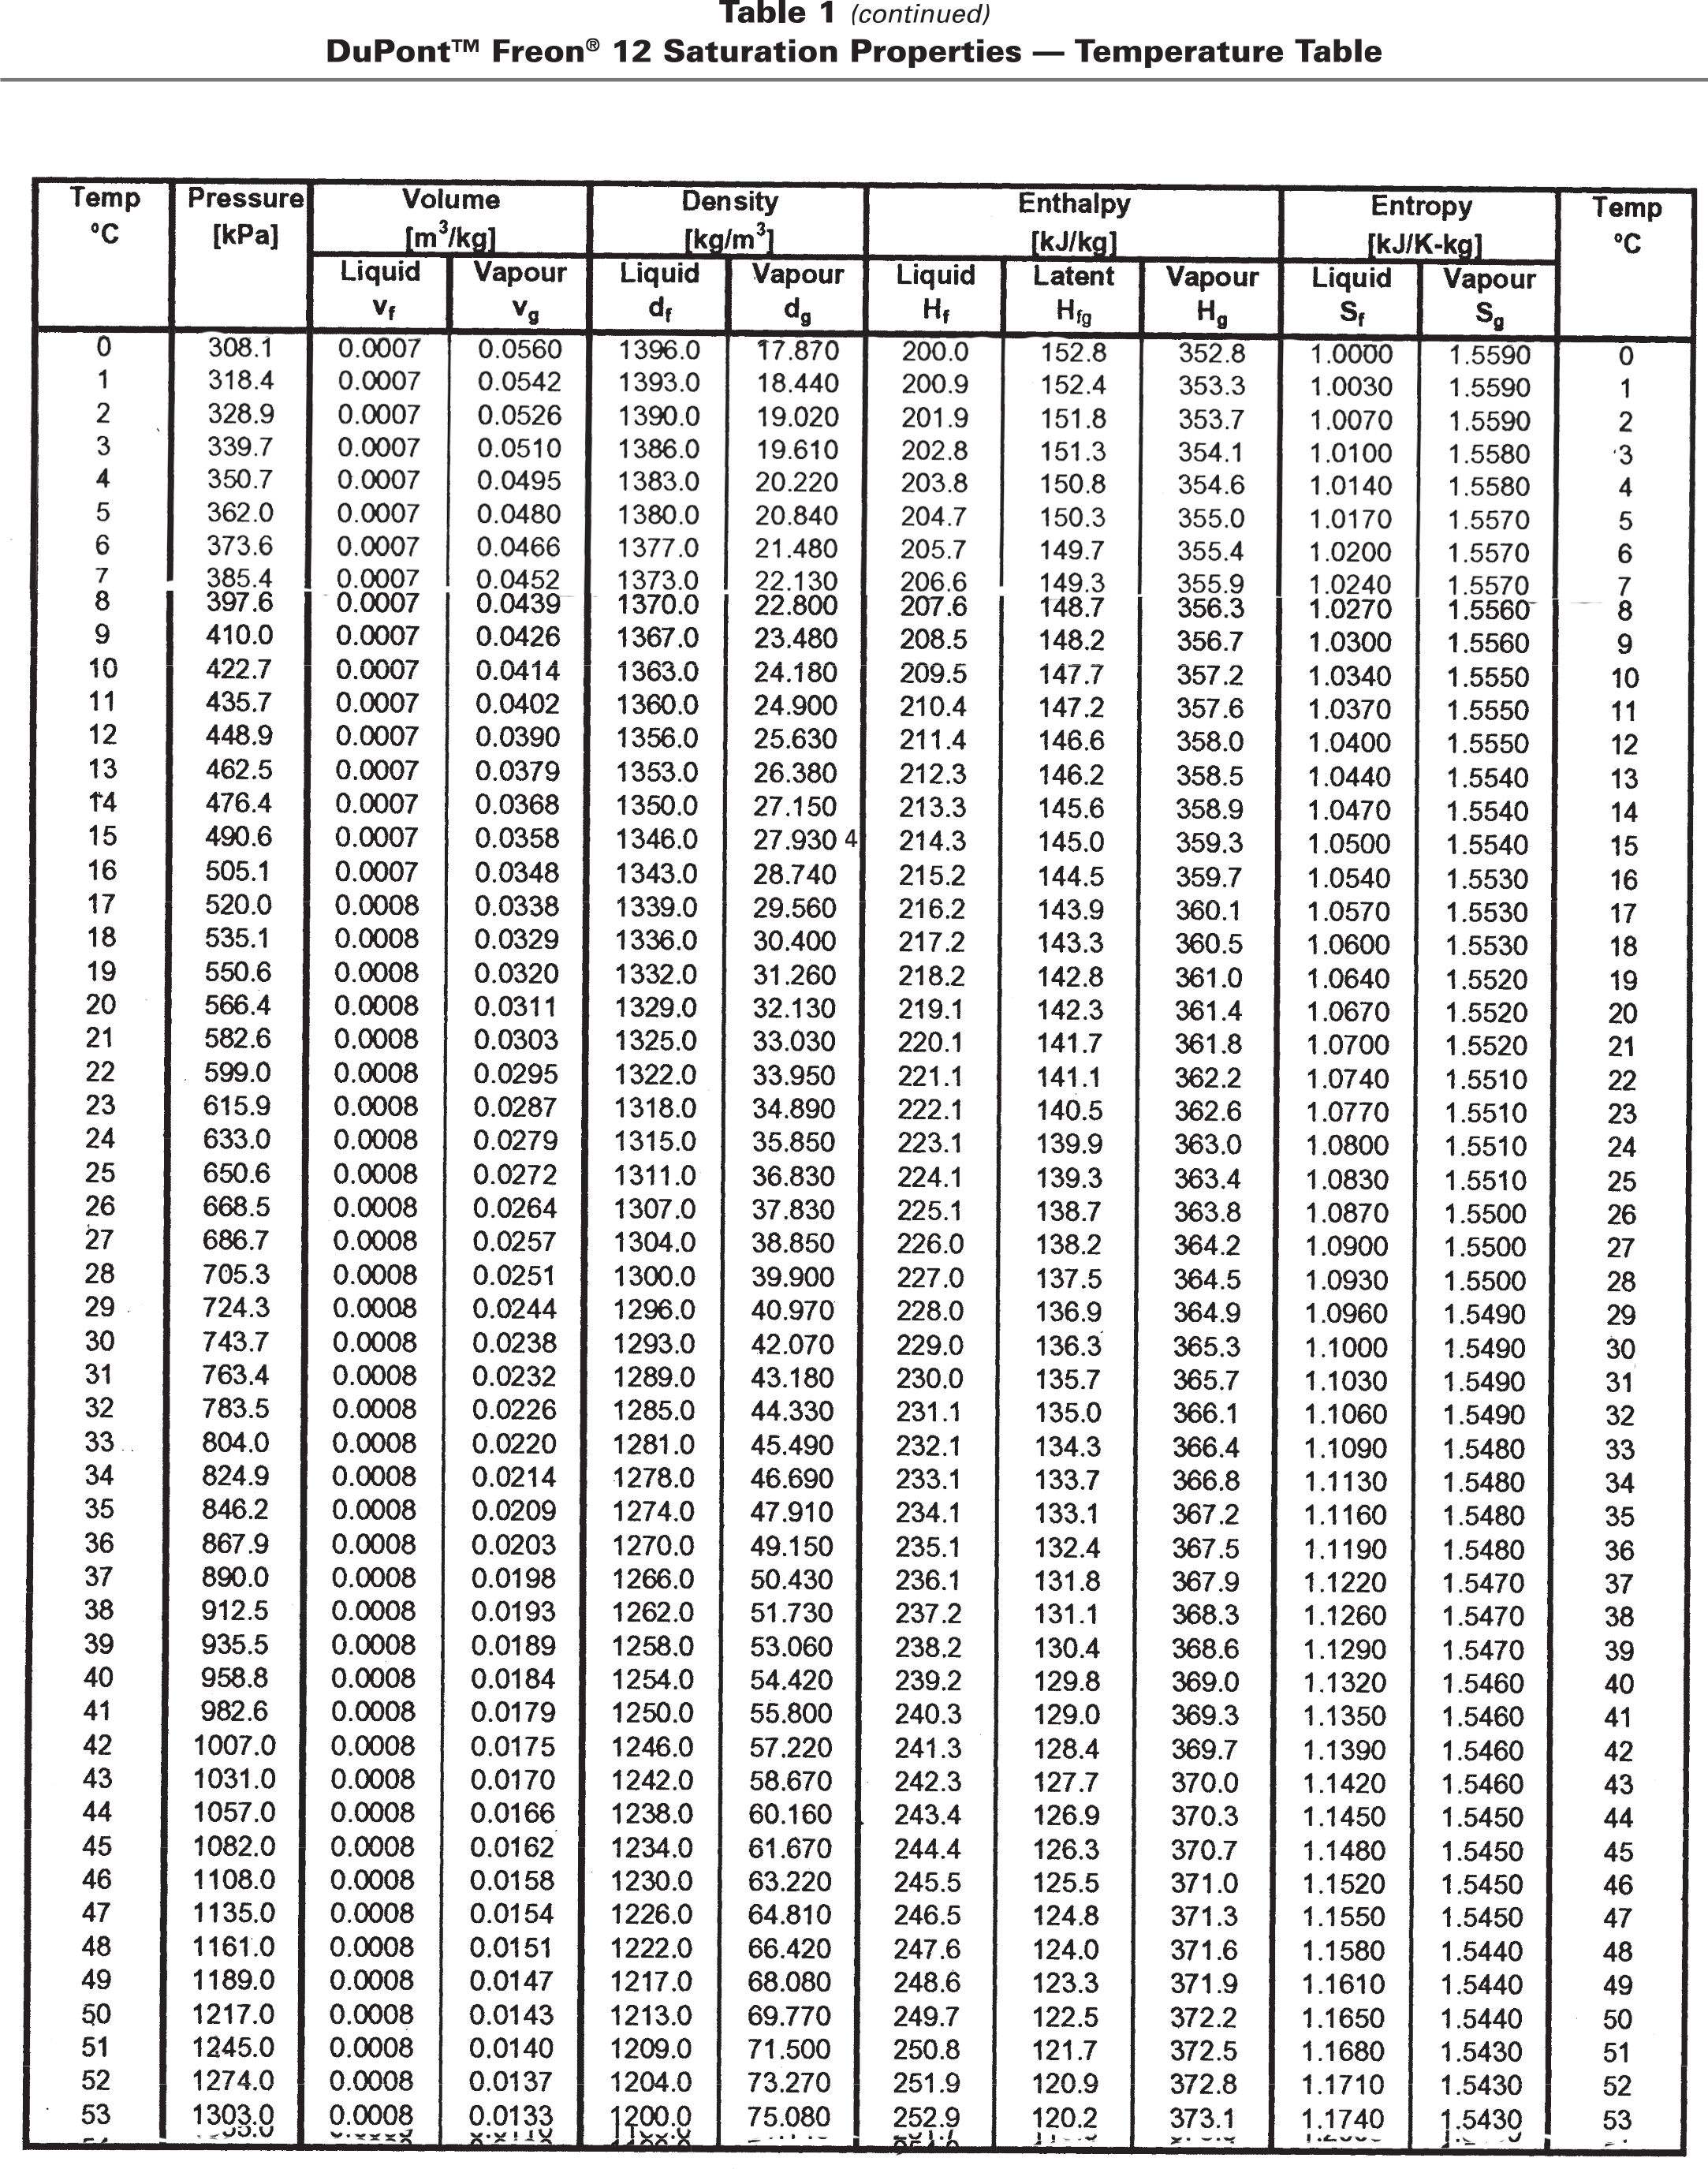
\includegraphics[width=0.9\linewidth]{TablaFreon12}
\end{table}

\begin{table}[H]
\centering
\caption[Tabla de vapor del Freón 12 (320-350{[}kPa{]})]{Tabla de vapor del Freón 12 (320-350{[}kPa{]})\cite{b:Tabla}}
\label{t:Freon12-340}
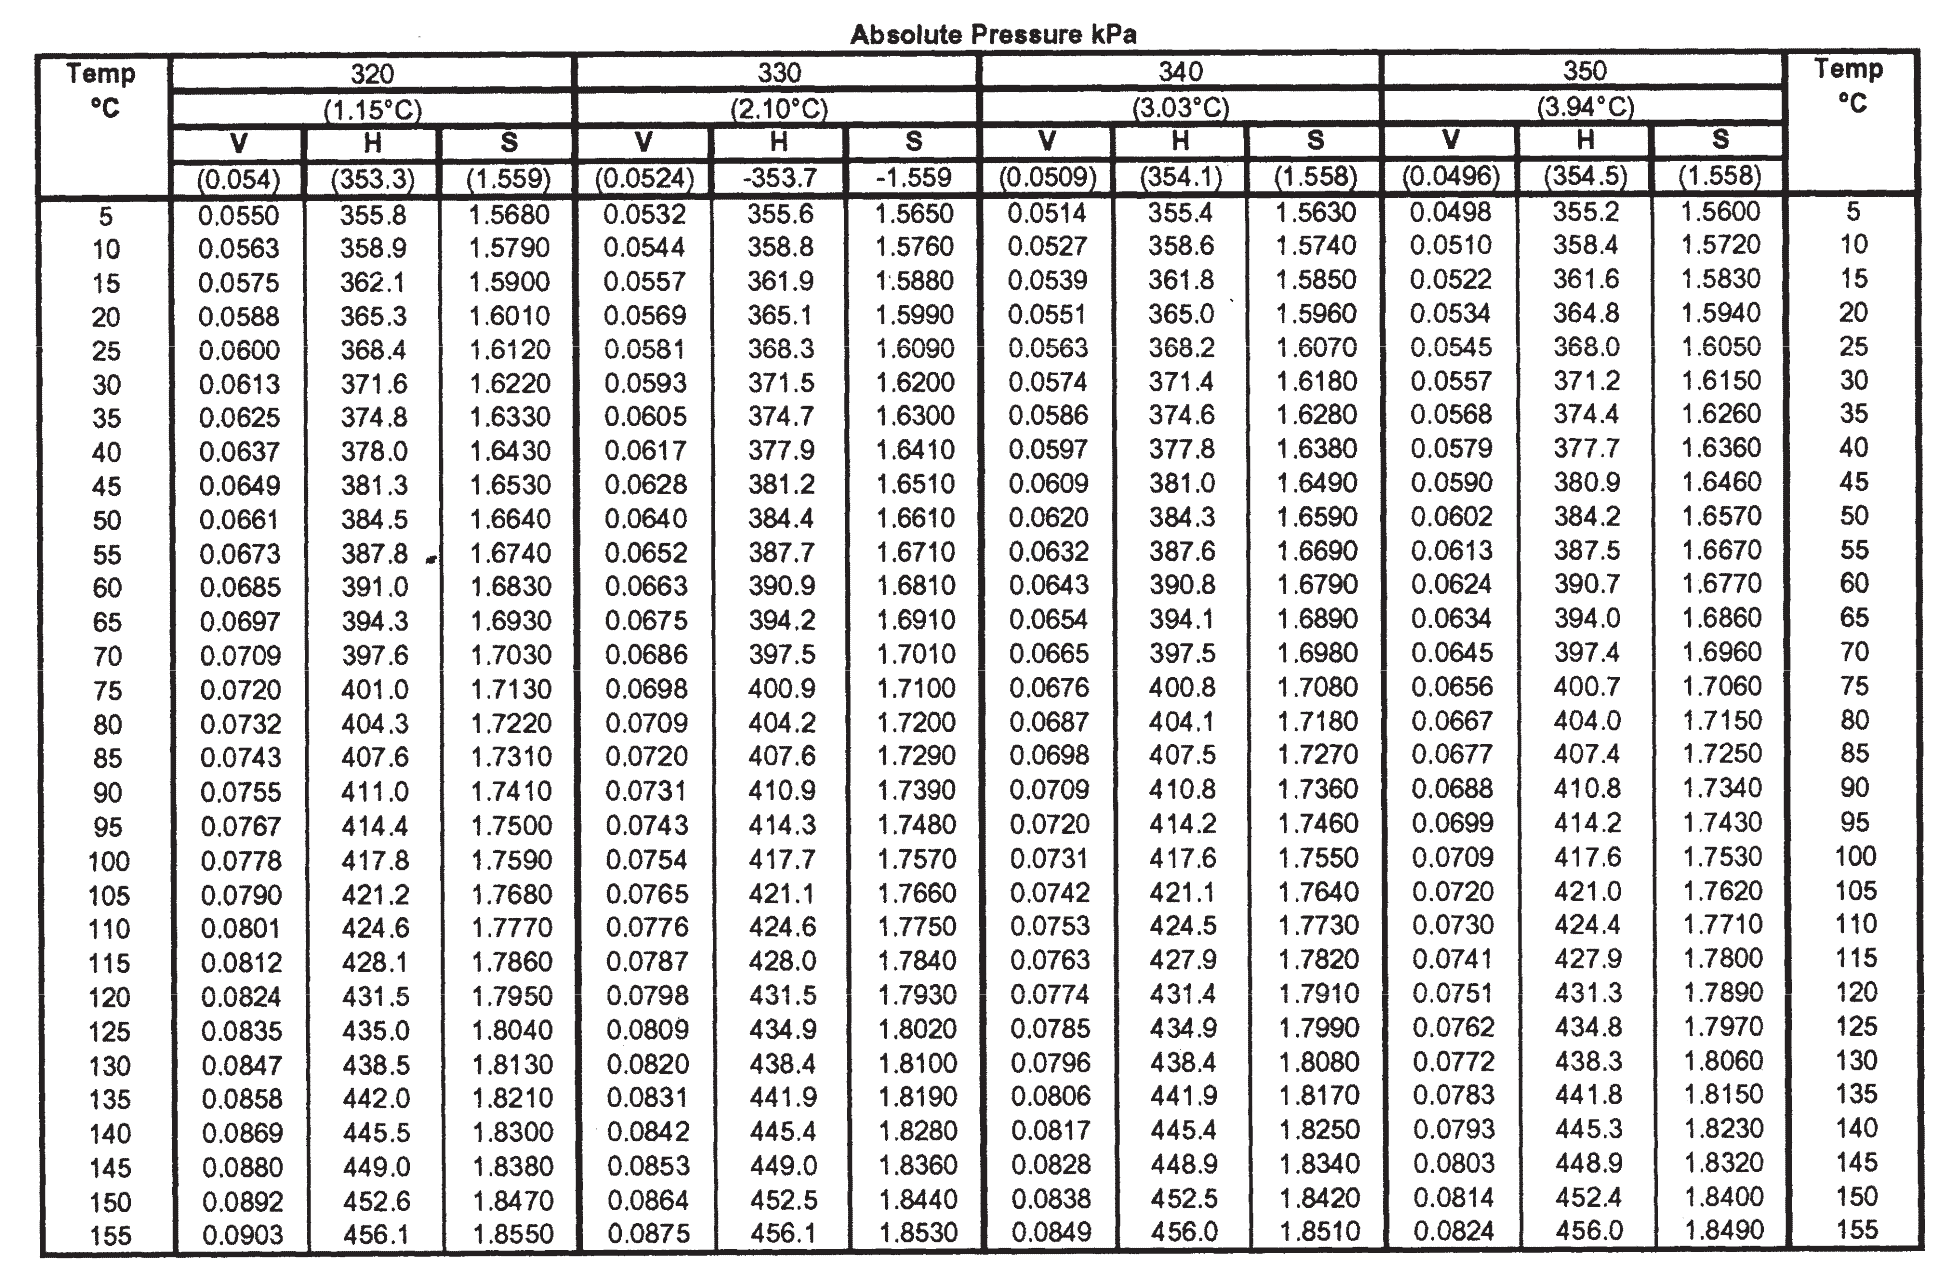
\includegraphics[width=0.85\linewidth]{TV-R12-340}
\end{table}


\begin{table}[H]
\centering
\caption[Tabla de vapor del Freón 12 (600-675{[}kPa{]})]{Tabla de vapor del Freón 12 (600-675{[}kPa{]})\cite{b:Tabla}}
\label{t:Freon12-700-1}
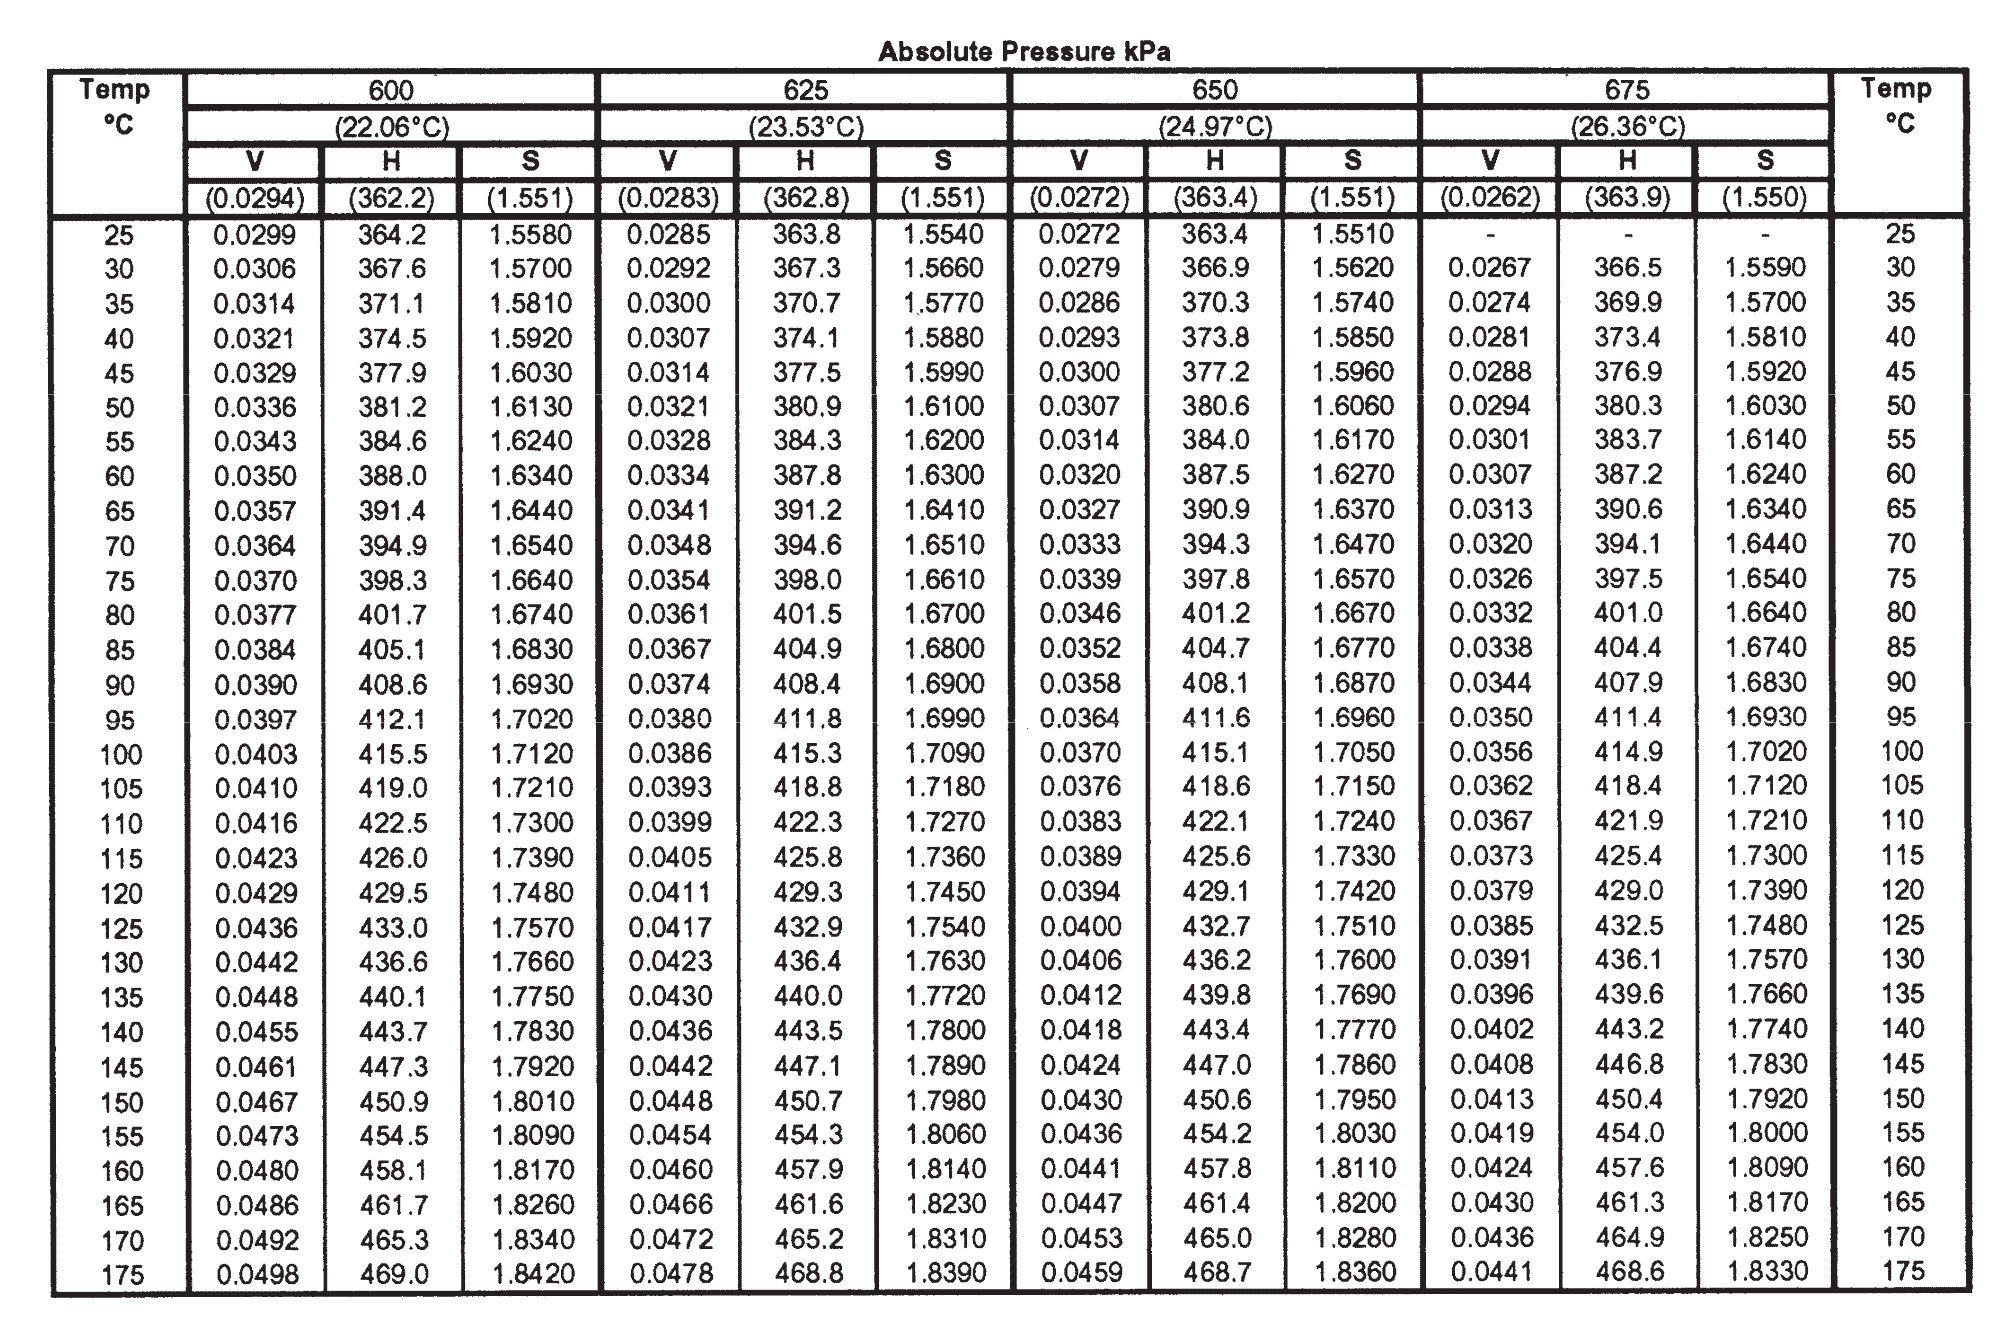
\includegraphics[width=0.85\linewidth]{TV-R12-700-1}
\end{table}

\begin{table}[H]
\centering
\caption[Tabla de vapor del Freón 12 (700-800{[}kPa{]})]{Tabla de vapor del Freón 12 (700-800[kPa])\cite{b:Tabla}}
\label{t:Freon12-700-2}
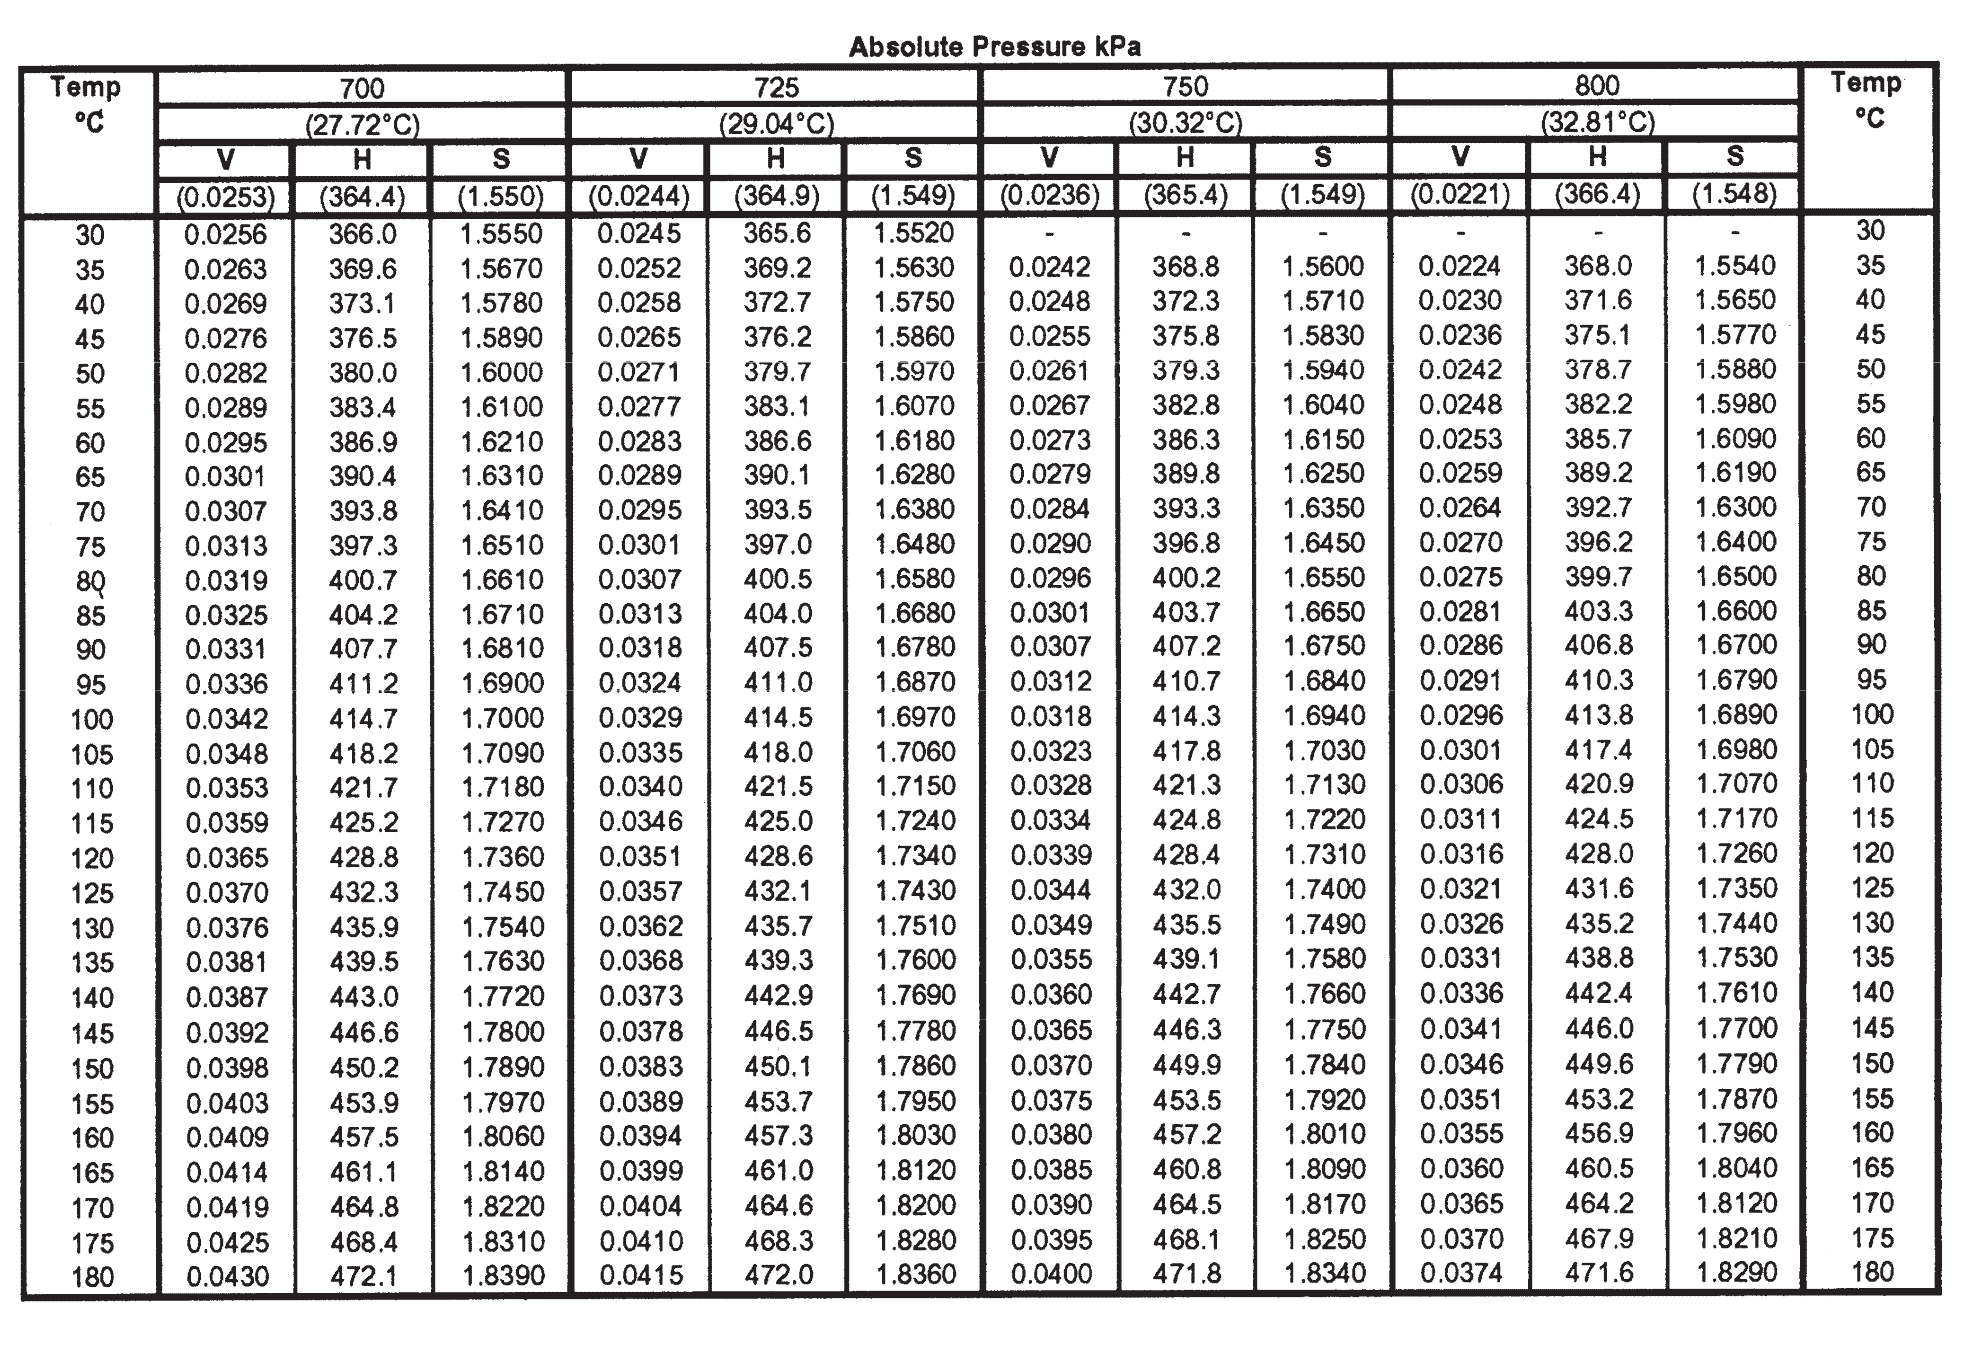
\includegraphics[width=\linewidth]{TV-R12-700-2}
\end{table}

\begin{table}[H]
\centering
\caption[Tabla de saturación del agua]{Tabla de saturación del agua\cite{b:Agua}}
\label{t:Agua}

\includegraphics[width=\linewidth]{Agua}
\end{table}














\begin{thebibliography}{x}
	\addcontentsline{toc}{section}{Referencias}
	
	\bibitem{b:Tabla} 
		DuPont. (2005). \textit{Thermodynamic Properties of DuPont Freon 12 Refrigerant.} E.E.U.U.
	
	\bibitem{b:Produccion}
W.H. Severns, H.E. Degler \& J.C. Miles. (1961). \textit{La Producción de energía mediante el vapor de agua, el aire y los gases.} New York: REVERTÉ.
	
	\bibitem{b:Agua}
	Y. A. ÇENGEL \& A. J. GHAJAR. (2007). \textit{Transferencia de calor y masa.} E.E.U.U.: Mc Graw Hill.
\end{thebibliography}

\end{document}

